\documentclass{beamer}

\usepackage{amsmath}
\usepackage{graphicx}

\usetheme{AnnArbor}
\usecolortheme{crane}
\usefonttheme[onlymath]{serif}

\title{Deep Learning - Foundations and Concepts}
\subtitle{Chapter 3. Standard Distributions}
\author{nonlineark@github}
\date{\today}

\begin{document}

\begin{frame}
    \titlepage
\end{frame}

\begin{frame}
    \frametitle{Outline}
    \tableofcontents
\end{frame}

\section{Discrete Variables}

\begin{frame}
    \frametitle{Bernoulli distribution}
    \begin{itemize}
        \item Consider a binary random variable $x\in\{0,1\}$ and a parameter $0\le\mu\le{}1$, such that $p(x=1)=\mu$ and $p(x=0)=1-\mu$.
        \item Probability distribution: $\mathrm{Bern}(x;\mu)=\mu^{x}(1-\mu)^{1-x}$.
        \item Expectation: $E(x)=\mu$.
        \item Variance: $\mathrm{var}(x)=\mu(1-\mu)$.
    \end{itemize}
\end{frame}

\begin{frame}
    \frametitle{Bernoulli distribution}
    Model the Bernoulli distribution given observations $\{x_{1},\hdots,x_{N}\}$.
    \begin{align*}
        p(x_{1},\hdots,x_{N};\mu)&=\prod_{n=1}^{N}\mu^{x_{n}}(1-\mu)^{1-x_{n}} \\
        \log{}p(x_{1},\hdots,x_{N};\mu)&=\sum_{n=1}^{N}(x_{n}\log\mu+(1-x_{n})\log(1-\mu)) \\
        &=\log\mu\sum_{n=1}^{N}x_{n}+\log(1-\mu)(N-\sum_{n=1}^{N}x_{n}) \\
        \mu_{ML}&=\frac{1}{N}\sum_{n=1}^{N}x_{n}
    \end{align*}
\end{frame}

\begin{frame}
    \frametitle{Binomial distribution}
    \begin{itemize}
        \item Consider a random variable $m=\sum_{n=1}^{N}x_{n}$, where $x_{n}$ are independent random variables obey Bernoulli distribution with parameter $\mu$.
        \item Probability distribution: $\mathrm{Bin}(m;N,\mu)={N\choose{}m}\mu^{m}(1-\mu)^{N-m}$.
        \item Expectation: $E(m)=N\mu$.
        \item Variance: $\mathrm{var}(m)=N\mu(1-\mu)$.
    \end{itemize}
\end{frame}

\begin{frame}
    \frametitle{Multinomial distribution}
    \begin{itemize}
        \item Consider a random variable $x\in\{\mathrm{e}_{1},\hdots,\mathrm{e}_{K}\}$ and a parameter $\mu\in\mathbb{R}^{K}$, such that $p(x=\mathrm{e}_{k})=\mu_{k}$.
        \item Probability distribution: $p(x;\mu)=\prod_{k=1}^{K}\mu_{k}^{x_{k}}$.
        \item Expectation: $E(x)=\mu$.
        \item Covariance: $\mathrm{cov}(x)=\mathrm{diag}(\mu_{1},\hdots,\mu_{K})-\mu\mu^{T}$.
    \end{itemize}
\end{frame}

\begin{frame}
    \frametitle{Multinomial distribution}
    Model the generalized Bernoulli distribution given observations $x^{1},\hdots,x^{N}$.
    \begin{align*}
        p(x^{1},\hdots,x^{N};\mu)&=\prod_{n=1}^{N}\prod_{k=1}^{K}\mu_{k}^{x^{n}_{k}} \\
        \log{}p(x^{1},\hdots,x^{N};\mu)&=\sum_{n=1}^{N}\sum_{k=1}^{K}x^{n}_{k}\log\mu_{k}=\sum_{k=1}^{K}(\sum_{n=1}^{N}x^{n}_{k})\log\mu_{k} \\
        \mu_{ML}&=\frac{1}{N}\sum_{n=1}^{N}x^{n}
    \end{align*}
    For the last step, we used Lagrange multiplier to take into the constraint $\sum_{k=1}^{K}\mu_{k}=1$.
\end{frame}

\begin{frame}
    \frametitle{Multinomial distribution}
    \begin{itemize}
        \item Consider a random variable $m=\sum_{n=1}^{N}x^{n}$, where $x^{n}$ are independent random variables obey the generalized Bernoulli distribution with parameter $\mu$.
        \item Probability distribution: $\mathrm{Mult}(m;N,\mu)=\frac{N!}{\prod_{k=1}^{K}m_{k}!}\prod_{k=1}^{K}\mu_{k}^{m_{k}}$.
        \item Expectation: $E(m)=N\mu$.
        \item Covariance: $\mathrm{cov}(m)=N(\mathrm{diag}(\mu_{1},\hdots,\mu_{K})-\mu\mu^{T})$.
    \end{itemize}
\end{frame}

\section{The Multivariate Gaussian}

\begin{frame}
    \frametitle{Definition}
    For a single variable $x$, the Gaussian distribution can be written in the form:
    \begin{equation*}
        \mathcal{N}(x;\mu,\sigma^{2})=\frac{1}{\sqrt{2\pi\sigma^{2}}}\exp(-\frac{(x-\mu)^{2}}{2\sigma^{2}})
    \end{equation*}
    where $\mu$ is the mean and $\sigma^{2}$ is the variance. For a $D$-dimensional vector $x$, the multivariate Gaussian distribution takes the form:
    \begin{equation*}
        \mathcal{N}(x;\mu,\Sigma)=\frac{1}{(2\pi)^{\frac{D}{2}}(\det\Sigma)^{\frac{1}{2}}}\exp(-\frac{1}{2}(x-\mu)^{T}\Sigma^{-1}(x-\mu))
    \end{equation*}
    where $\mu$ is the $D$-dimensional mean vector, $\Sigma$ is the $D\times{}D$ covariance matrix.
\end{frame}

\begin{frame}
    \frametitle{Geometry of the Gaussian}
    Without loss of generality, we assume $\Sigma$ is symmetric. As a self-adjoint operator, there exists an orthonormal basis $(u_{1},\hdots,u_{D})$ under which $\Sigma$ is diagonalized:
    \begin{equation*}
        \mathrm{diag}(\lambda_{1},\hdots,\lambda_{D})=U^{T}\Sigma{}U
    \end{equation*}
    where $U$ is the orthogonal matrix whose $j$th column is $u_{j}$. Now let $x-\mu=Uy$, we see that under the new basis, the multivariate Gaussian takes the form:
    \begin{align*}
        \mathcal{N}(x;\mu,\Sigma)&=\frac{1}{(2\pi)^{\frac{D}{2}}(\lambda_{1}\hdots\lambda_{D})^{\frac{1}{2}}}\exp(-\frac{1}{2}y^{T}\mathrm{diag}^{-1}(\lambda_{1},\hdots,\lambda_{D})y)|\det{}U| \\
        &=\frac{1}{\sqrt{2\pi\lambda_{1}}\hdots\sqrt{2\pi\lambda_{D}}}\exp(-\frac{1}{2}\sum_{d=1}^{D}\frac{y_{d}^{2}}{\lambda_{d}}) \\
        &=\prod_{d=1}^{D}\frac{1}{\sqrt{2\pi\lambda_{d}}}\exp(-\frac{y_{d}^{2}}{2\lambda_{d}})
    \end{align*}
\end{frame}

\begin{frame}
    \frametitle{Geometry of the Gaussian}
    \begin{figure}
        \caption{Geometry of the Gaussian}
        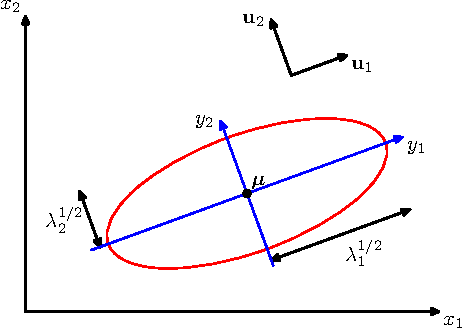
\includegraphics{Figure_3.pdf}
    \end{figure}
\end{frame}

\begin{frame}
    \frametitle{Geometry of the Gaussian}
    It's easy to see that the multivariate Gaussian is indeed normalized:
    \begin{align*}
        \int\mathcal{N}(x;\mu,\Sigma)\mathrm{d}x&=\int\prod_{d=1}^{D}\frac{1}{\sqrt{2\pi\lambda_{d}}}\exp(-\frac{y_{d}^{2}}{2\lambda_{d}})\mathrm{d}y \\
        &=\prod_{d=1}^{D}\int_{-\infty}^{+\infty}\frac{1}{\sqrt{2\pi\lambda_{d}}}\exp(-\frac{y_{d}^{2}}{2\lambda_{d}})\mathrm{d}y_{d} \\
        &=1
    \end{align*}
\end{frame}

\begin{frame}
    \frametitle{Expectation and covariance}
    Similarly, we can calculate the expectation and covariance of the multivariate Gaussian:
    \begin{align*}
        E(x)&=\int\mathcal{N}(x;\mu,\Sigma)x\mathrm{d}x \\
        &=\int\prod_{d=1}^{D}\frac{1}{\sqrt{2\pi\lambda_{d}}}\exp(-\frac{y_{d}^{2}}{2\lambda_{d}})(\mu+Uy)|\det{}U|\mathrm{d}y \\
        &=\mu+U\int\prod_{d=1}^{D}\frac{1}{\sqrt{2\pi\lambda_{d}}}\exp(-\frac{y_{d}^{2}}{2\lambda_{d}})y\mathrm{d}y \\
        &=\mu
    \end{align*}
\end{frame}

\begin{frame}
    \frametitle{Expectation and covariance}
    \begin{align*}
        E(xx^{T})&=\int\mathcal{N}(x;\mu,\Sigma)xx^{T}\mathrm{d}x \\
        &=\int\prod_{d=1}^{D}\frac{1}{\sqrt{2\pi\lambda_{d}}}\exp(-\frac{y_{d}^{2}}{2\lambda_{d}})(\mu+Uy)(\mu+Uy)^{T}|\det{}U|\mathrm{d}y \\
        &=\mu\mu^{T}+U(\int\prod_{d=1}^{D}\frac{1}{\sqrt{2\pi\lambda_{d}}}\exp(-\frac{y_{d}^{2}}{2\lambda_{d}})yy^{T}\mathrm{d}y)U^{T} \\
        &=\mu\mu^{T}+U\mathrm{diag}(\lambda_{1},\hdots,\lambda_{D})U^{T}=\mu\mu^{T}+\Sigma \\
        \mathrm{cov}(x)&=E(xx^{T})-E(x)E(x^{T})=\Sigma
    \end{align*}
\end{frame}

\begin{frame}
    \frametitle{The good and the bad about the Gaussian}
    \begin{itemize}
        \item The Gaussian distribution arises in many different contexts:
        \begin{itemize}
            \item The distribution that maximizes the entropy is the Gaussian.
            \item Central limit theorem.
        \end{itemize}
        \item The Gaussian distribution has many important analytical properties.
        \item For large $D$, the total number of parameters grows quadratically with $D$, manipulating and inverting the large matrices can become prohibitive.
        \item The Gaussian distribution is intrinsically unimodal, and so is unable to provide a good approximation to multimodal distributions.
    \end{itemize}
\end{frame}

\begin{frame}
    \frametitle{Conditional distribution and marginal distribution}
    \begin{block}{Problem}
        Suppose $x$ obeys the Gaussian distribution $\mathcal{N}(x;\mu,\Sigma)$. If we partition $x$ into $x_{a}$ and $x_{b}$, that is $x=\begin{pmatrix}
            x_{a} \\
            x_{b}
        \end{pmatrix}$, what are the expressions for the conditional distribution $p(x_{a}|x_{b})$ and the marginal distribution $p(x_{a})$?
    \end{block}
\end{frame}

\begin{frame}
    \frametitle{Conditional distribution and marginal distribution}
    First step, let's also partition the mean and covariance accordingly:
    \begin{align*}
        \mu&=\begin{pmatrix}
            \mu_{a} \\
            \mu_{b}
        \end{pmatrix} \\
        \Sigma&=\begin{pmatrix}
            \Sigma_{aa}&\Sigma_{ab} \\
            \Sigma_{ba}&\Sigma_{bb}
        \end{pmatrix}
    \end{align*}
    Because $\Sigma^{-1}$ (called the precision matrix) appears frequently, we also partition $\Sigma^{-1}$:
    \begin{equation*}
        \Sigma^{-1}=\begin{pmatrix}
            \Lambda_{aa}&\Lambda_{ab} \\
            \Lambda_{ba}&\Lambda_{bb}
        \end{pmatrix}
    \end{equation*}
    Notice that because $\Sigma$ and $\Sigma^{-1}$ are symmetric, $\Sigma_{aa}$, $\Sigma_{bb}$, $\Lambda_{aa}$ and $\Lambda_{bb}$ are symmetric as well. Further, we have $\Sigma_{ba}=\Sigma_{ab}^{T}$ and $\Lambda_{ba}=\Lambda_{ab}^{T}$.
\end{frame}

\begin{frame}
    \frametitle{Conditional distribution and marginal distribution}
    Second step, let's complete the square! Notice:
    \begin{equation*}
        (x-\mu)^{T}\Sigma^{-1}(x-\mu)=x\Sigma^{-1}x-2x^{T}\Sigma^{-1}\mu+\mu^{T}\Sigma^{-1}\mu
    \end{equation*}
    For conditional distribution $p(x_{a}|x_{b})$:
    \begin{align*}
        (x-\mu)^{T}\Sigma^{-1}(x-\mu)&=\begin{pmatrix}
            x_{a}^{T}-\mu_{a}^{T}&x_{b}^{T}-\mu_{b}^{T}
        \end{pmatrix}
        \begin{pmatrix}
            \Lambda_{aa}&\Lambda_{ab} \\
            \Lambda_{ba}&\Lambda_{bb}
        \end{pmatrix}
        \begin{pmatrix}
            x_{a}-\mu_{a} \\
            x_{b}-\mu_{b}
        \end{pmatrix} \\
        &=x_{a}^{T}\Lambda_{aa}x_{a}-2x_{a}^{T}(\Lambda_{aa}\mu_{a}-\Lambda_{ab}(x_{b}-\mu_{b}))+\mathrm{const}
    \end{align*}
    Compare, we see:
    \begin{align*}
        \Sigma_{x_{a}|x_{b}}^{-1}&=\Lambda_{aa} \\
        \Sigma_{x_{a}|x_{b}}&=\Lambda_{aa}^{-1} \\
        \Sigma_{x_{a}|x_{b}}^{-1}\mu_{x_{a}|x_{b}}&=\Lambda_{aa}\mu_{a}-\Lambda_{ab}(x_{b}-\mu_{b}) \\
        \mu_{x_{a}|x_{b}}&=\mu_{a}-\Lambda_{aa}^{-1}\Lambda_{ab}(x_{b}-\mu_{b})
    \end{align*}
\end{frame}

\begin{frame}
    \frametitle{Conditional distribution and marginal distribution}
    For marginal distribution, $p(x_{a})=\int{}p(x_{a},x_{b})\mathrm{d}x_{b}$. Let's first complete the square for $x_{b}$ to integrate it out:
    \begin{align*}
        &(x-\mu)^{T}\Sigma^{-1}(x-\mu)=\begin{pmatrix}
            x_{a}^{T}-\mu_{a}^{T}&x_{b}^{T}-\mu_{b}^{T}
        \end{pmatrix}
        \begin{pmatrix}
            \Lambda_{aa}&\Lambda_{ab} \\
            \Lambda_{ba}&\Lambda_{bb}
        \end{pmatrix}
        \begin{pmatrix}
            x_{a}-\mu_{a} \\
            x_{b}-\mu_{b}
        \end{pmatrix} \\
        &=x_{b}^{T}\Lambda_{bb}x_{b}-2x_{b}^{T}\Lambda_{bb}(\mu_{b}-\Lambda_{bb}^{-1}\Lambda_{ba}(x_{a}-\mu_{a}))+\cdots \\
        &=x_{b}^{T}\Lambda_{bb}x_{b}-2x_{b}^{T}\Lambda_{bb}m+m^{T}\Lambda_{bb}m+\cdots \\
        &=(x_{b}-m)^{T}\Lambda_{bb}(x_{b}-m)+\cdots
    \end{align*}
    where $m=\mu_{b}-\Lambda_{bb}^{-1}\Lambda_{ba}(x_{a}-\mu_{a})$. We see that when integrating $x_{b}$, the result will be a constant not depending on $x_{a}$, although $m$ depends on $x_{a}$.
\end{frame}

\begin{frame}
    \frametitle{Conditional distribution and marginal distribution}
    Which means, we can take a look at the terms left in $\cdots$, and complete the square for $x_{a}$ to get the mean and the covariance for $x_{a}$:
    \begin{equation*}
        \cdots=(x_{a}-\mu_{a})^{T}(\Lambda_{aa}-\Lambda_{ab}\Lambda_{bb}^{-1}\Lambda_{ba})(x_{a}-\mu_{a})
    \end{equation*}
    We see that:
    \begin{align*}
        \Sigma_{x_{a}}&=(\Lambda_{aa}-\Lambda_{ab}\Lambda_{bb}^{-1}\Lambda_{ba})^{-1} \\
        \mu_{x_{a}}&=\mu_{a}
    \end{align*}
    Through a rather ugly equation (known as \href{https://en.wikipedia.org/wiki/Schur_complement}{Schur complement}), we can simplify the expression for $\Sigma_{x_{a}}$ to a much nicer one:
    \begin{equation*}
        \Sigma_{x_{a}}=\Sigma_{aa}
    \end{equation*}
\end{frame}

\begin{frame}
    \frametitle{Conditional distribution and marginal distribution}
    \begin{figure}
        \caption{The marginal distribution and the conditional distribution}
        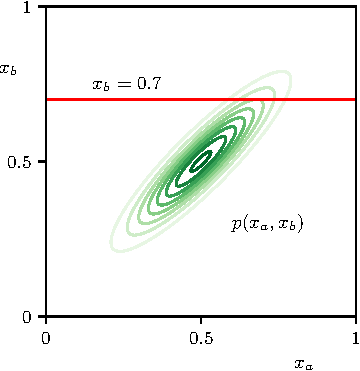
\includegraphics[width=0.4\textwidth]{Figure_5_a.pdf}
        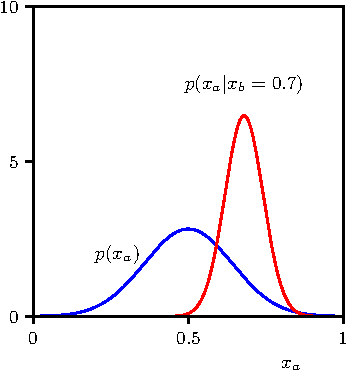
\includegraphics[width=0.4\textwidth]{Figure_5_b.pdf}
    \end{figure}
\end{frame}

\begin{frame}
    \frametitle{Bayes' theorem}
    \begin{block}{Problem}
        Suppose that we are given a Gaussian marginal distribution $p(x)$ and a Gaussian conditional distribution $p(y|x)$. What are the expressions for the marginal distribution $p(y)$ and the conditional distribution $p(x|y)$?
    \end{block}
\end{frame}

\begin{frame}
    \frametitle{Bayes' theorem}
    To make things easier, we suppose that $p(y|x)$ has a mean that is a linear function of $x$ and a covariance that is independent of $x$:
    \begin{align*}
        p(x)&=\mathcal{N}(x;\mu,\Lambda^{-1}) \\
        p(y|x)&=\mathcal{N}(y;Ax+b,L^{-1})
    \end{align*}
\end{frame}

\begin{frame}
    \frametitle{Bayes' theorem}
    Let's find the joint distribution of $p(x,y)$, then from $p(x,y)$ we can easily get both $p(y)$ and $p(x|y)$:
    \begin{align*}
        &(x-\mu)^{T}\Lambda(x-\mu)+(y-(Ax+b))^{T}L(y-(Ax+b)) \\
        &=\begin{pmatrix}
            x \\
            y
        \end{pmatrix}^{T}
        \begin{pmatrix}
            \Lambda+A^{T}LA&-A^{T}L \\
            -LA&L
        \end{pmatrix}
        \begin{pmatrix}
            x \\
            y
        \end{pmatrix}
        -2\begin{pmatrix}
            x \\
            y
        \end{pmatrix}^{T}
        \begin{pmatrix}
            \Lambda\mu-A^{T}Lb \\
            Lb
        \end{pmatrix}
    \end{align*}
    Using the (ugly but useful) Schur complement again, we have:
    \begin{align*}
        \Lambda_{x,y}&=\begin{pmatrix}
            \Lambda+A^{T}LA&-A^{T}L \\
            -LA&L
        \end{pmatrix} \\
        \Sigma_{x,y}&=\Lambda_{x,y}^{-1}=\begin{pmatrix}
            \Lambda^{-1}&\Lambda^{-1}A^{T} \\
            A\Lambda^{-1}&L^{-1}+A\Lambda^{-1}A^{T}
        \end{pmatrix} \\
        \mu_{x,y}&=\Sigma_{x,y}\begin{pmatrix}
            \Lambda\mu-A^{T}Lb \\
            Lb
        \end{pmatrix}=\begin{pmatrix}
            \mu \\
            A\mu+b
        \end{pmatrix}
    \end{align*}
\end{frame}

\begin{frame}
    \frametitle{Bayes' theorem}
    From the joint distribution of $p(x,y)$, we can easily get:
    \begin{align*}
        \Sigma_{y}&=L^{-1}+A\Lambda^{-1}A^{T} \\
        \mu_{y}&=A\mu+b \\
        \Lambda_{x|y}&=\Lambda+A^{T}LA \\
        \mu_{x|y}&=\mu-(\Lambda+A^{T}LA)^{-1}(-A^{T}L)(y-(A\mu+b)) \\
        &=(\Lambda+A^{T}LA)^{-1}(A^{T}L(y-b)+\Lambda\mu)
    \end{align*}
\end{frame}

\begin{frame}
    \frametitle{Maximum likelihood}
    \begin{block}{Problem}
        We have $N$ observations of a random variable $x$: $x_{1},\hdots,x_{N}$ that are drawn independently from a multivariate Gaussian distribution whose mean $\mu$ and covariance $\Sigma$ are unknown. How do we determine these parameters from the data set?
    \end{block}
\end{frame}

\begin{frame}
    \frametitle{Maximum likelihood}
    \begin{align*}
        L&=-\log{}p(x_{1},\hdots,x_{N};\mu,\Lambda^{-1}) \\
        &=\frac{ND}{2}\log(2\pi)-\frac{N}{2}\log\det\Lambda+\frac{1}{2}\sum_{n=1}^{N}(x_{n}-\mu)^{T}\Lambda(x_{n}-\mu) \\
        \frac{\partial{}L}{\partial\mu}&=N(\mu-\frac{1}{N}\sum_{n=1}^{N}x_{n})^{T}\Lambda\qquad\mu_{ML}=\frac{1}{N}\sum_{n=1}^{N}x_{n} \\
        \frac{\partial{}L}{\partial\Lambda}(\Lambda)H&=\frac{N}{2}\mathrm{tr}((\frac{1}{N}\sum_{n=1}^{N}(x_{n}-\mu)(x_{n}-\mu)^{T}-\Lambda^{-1})H) \\
        \Sigma_{ML}&=\Lambda^{-1}_{ML}=\frac{1}{N}\sum_{n=1}^{N}(x_{n}-\mu_{ML})(x_{n}-\mu_{ML})^{T}
    \end{align*}
\end{frame}

\begin{frame}
    \frametitle{Maximum likelihood}
    A couple of more words regarding $\frac{\partial{}L}{\partial\Lambda}$. The only thing that needs more explanation is how to differentiate $\log\det{}X$:
    \begin{equation*}
        \lim_{h\to{}0}\frac{1}{h}(\det(X+h\mathrm{e}_{ij})-\det{}X)=\lim_{h\to{}0}\frac{1}{h}(\det{}X+hX_{ij}-\det{}X)=X_{ij}
    \end{equation*}
    where $X_{ij}$ is the $ij$-cofactor of $X$. Now we can calculate $D\det$ easily:
    \begin{equation*}
        D\det{}(X)H=\sum_{i,j}X_{ij}h_{ij}=\mathrm{tr}((\mathrm{cof}(X))^{T}H)
    \end{equation*}
    where $\mathrm{cof}(X)$ is the cofactor matrix of $X$. From here we have:
    \begin{equation*}
        D\log\det{}(X)H=\frac{1}{\det{}X}D\det{}(X)H=\frac{1}{\det{}X}\mathrm{tr}((\mathrm{cof}X)^{T}H)=\mathrm{tr}(X^{-1}H)
    \end{equation*}
\end{frame}

\begin{frame}
    \frametitle{Maximum likelihood}
    Similarly to univariate Gaussian, we find that $\Sigma_{ML}$ is biased:
    \begin{align*}
        E(\mu_{ML})&=\mu \\
        E(\Sigma_{ML})&=\frac{N-1}{N}\Sigma
    \end{align*}
    We can correct this bias by defining a different estimator $\tilde{\Sigma}$ given by:
    \begin{equation*}
        \tilde{\Sigma}=\frac{1}{N-1}\sum_{n=1}^{N}(x_{n}-\mu_{ML})(x_{n}-\mu_{ML})^{T}
    \end{equation*}
\end{frame}

\begin{frame}
    \frametitle{Sequential estimation}
    Because $\mu_{ML}$ only depends on the sum of the data points, it allows us to process the data points one at a time. If we denote by $\mu_{ML}^{N}$ the result for the maximum likelihood estimator of the mean when it is based on $N$ observations:
    \begin{align*}
        \mu_{ML}^{N}&=\frac{1}{N}\sum_{n=1}^{N}x_{n} \\
        &=\frac{1}{N}((N-1)\mu_{ML}^{N-1}+x_{N}) \\
        &=\mu_{ML}^{N-1}+\frac{1}{N}(x_{N}-\mu_{ML}^{N-1})
    \end{align*}
\end{frame}

\begin{frame}
    \frametitle{Mixtures of Gaussians}
    \begin{figure}
        \caption{A single Gaussian fails to capture the two clumps while a linear combination of two Gaussians gives a better representation}
        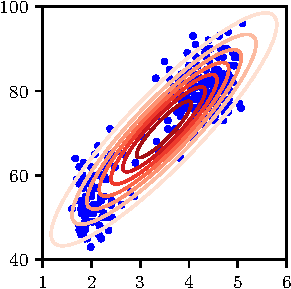
\includegraphics[width=0.4\textwidth]{Figure_6_a.pdf}
        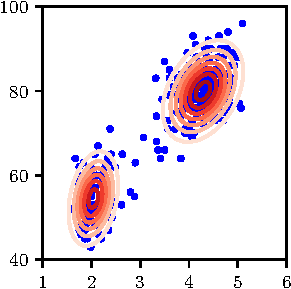
\includegraphics[width=0.4\textwidth]{Figure_6_b.pdf}
    \end{figure}
\end{frame}

\begin{frame}
    \frametitle{Mixtures of Gaussians}
    A mixture of Gaussians is a superposition of $K$ Gaussian densities:
    \begin{equation*}
        p(x)=\sum_{k=1}^{K}\pi_{k}\mathcal{N}(x;\mu_{k},\Sigma_{k})
    \end{equation*}
    where $0\le\pi_{k}\le{}1$ and $\sum_{k=1}^{K}\pi_{k}=1$.
    \begin{figure}
        \caption{Example of a Gaussian mixture distribution}
        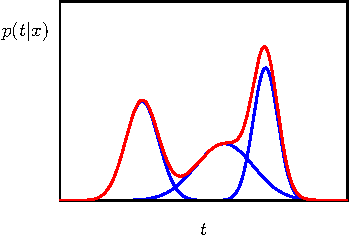
\includegraphics{Figure_7.pdf}
    \end{figure}
\end{frame}

\section{Periodic Variables}

\begin{frame}
    \frametitle{Periodic variables}
    \begin{block}{Problem}
        Evaluating the mean of a set of observations $\{\theta_{1},\hdots,\theta_{N}\}$ of a periodic variable $\theta$ where $\theta$ is measured in radians.
    \end{block}
\end{frame}

\begin{frame}
    \frametitle{Periodic variables}
    Consider this as a 2-dimensional problem instead of a 1-dimensional one. Each $\theta_{n}$ corresponds to a point $x_{n}$ on the unit circle, let's find the angle $\bar{\theta}$ for the average of these points $\bar{x}$:
    \begin{align*}
        \bar{x}&=\frac{1}{N}\sum_{n=1}^{N}x_{n}=\frac{1}{N}\sum_{n=1}^{N}\begin{pmatrix}
            \cos\theta_{n} \\
            \sin\theta_{n}
        \end{pmatrix}
        =\begin{pmatrix}
            \frac{1}{N}\sum_{n=1}^{N}\cos\theta_{n} \\
            \frac{1}{N}\sum_{n=1}^{N}\sin\theta_{n}
        \end{pmatrix} \\
        \tan\bar{\theta}&=\frac{\sum_{n=1}^{N}\sin\theta_{n}}{\sum_{n=1}^{N}\cos\theta_{n}}
    \end{align*}
\end{frame}

\begin{frame}
    \frametitle{Von Mises distribution}
    Periodic probability density:
    \begin{align*}
        p(\theta)&\ge{}0 \\
        \int_{0}^{2\pi}p(\theta)\mathrm{d}\theta&=1 \\
        p(\theta+2\pi)&=p(\theta)
    \end{align*}
    Is there a periodic probability density $p(\theta)$ that gives the result $\tan\bar{\theta}=\frac{\sum_{n=1}^{N}\sin\theta_{n}}{\sum_{n=1}^{N}\cos\theta_{n}}$ as a maximum likelihood estimator?
\end{frame}

\begin{frame}
    \frametitle{Von Mises distribution}
    Let's consider a 2-dimensional Gaussian conditioning on the unit circle, where the mean $\mu=\begin{pmatrix}
        \mu_{1}  \\
        \mu_{2}
    \end{pmatrix}=r_{0}
    \begin{pmatrix}
        \cos\theta_{0} \\
        \sin\theta_{0}
    \end{pmatrix}$ and the covariance $\Sigma=\sigma^{2}I$:
    \begin{align*}
        p(x_{1},x_{2})&=\frac{1}{2\pi\sigma^{2}}\exp(-\frac{(x_{1}-\mu_{1})^{2}+(x_{2}-\mu_{2})^{2}}{2\sigma^{2}}) \\
        p(r,\theta)&=\frac{1}{2\pi\sigma^{2}}\exp(-\frac{r^{2}-2r_{0}r\cos(\theta-\theta_{0})+r_{0}^{2}}{2\sigma^{2}})r \\
        p(\theta|r=1)&=C\exp(\frac{r_{0}}{\sigma^{2}}\cos(\theta-\theta_{0}))
    \end{align*}
    Let $m=\frac{r_{0}}{\sigma^{2}}$, and normalize the constant $C$, we have:
    \begin{equation*}
        p(\theta;\theta_{0},m)=\frac{1}{2\pi{}I_{0}(m)}\exp(m\cos(\theta-\theta_{0}))
    \end{equation*}
\end{frame}

\begin{frame}
    \frametitle{Von Mises distribution}
    Let's consider the maximum likelihood estimator for the parameter $\theta_{0}$:
    \begin{align*}
        L&=\log{}p(\theta_{1},\hdots,\theta_{N};\theta_{0},m) \\
        &=-N\log(2\pi{}I_{0}(m))+m\sum_{n=1}^{N}\cos(\theta_{n}-\theta_{0}) \\
        \frac{\partial{}L}{\partial\theta_{0}}&=m\sum_{n=1}^{N}\sin(\theta_{n}-\theta_{0})=m(\cos\theta_{0}\sum_{n=1}^{N}\sin\theta_{n}-\sin\theta_{0}\sum_{n=1}^{N}\cos\theta_{n})
    \end{align*}
    We indeed have:
    \begin{equation*}
        \theta_{0}^{ML}=\frac{\sum_{n=1}^{N}\sin\theta_{n}}{\sum_{n=1}^{N}\cos\theta_{n}}
    \end{equation*}
\end{frame}

\end{document}